%%「論文」,「レター」,「レター(C分冊)」,「技術研究報告」などのテンプレート
%% v3.3N [2023/03/30]
%% 1. 「論文」
\documentclass[paper]{ieicej}
%\documentclass[invited]{ieicej}% 招待論文
%\documentclass[survey]{ieicej}% サーベイ論文
%\documentclass[comment]{ieicej}% 解説論文
% \usepackage[dvips]{graphicx}
\usepackage[dvipdfmx]{graphicx,xcolor}
\usepackage[fleqn]{amsmath}
\usepackage{newtxtext}% 英数字フォントの設定を変更しないでください
\usepackage[varg]{newtxmath}% % 英数字フォントの設定を変更しないでください
\usepackage{latexsym}
\usepackage{multirow}
\usepackage{url}	% \url{}コマンド用.URLを表示する際に便利

\newcommand{\todo}[1]{\colorbox{yellow}{{\bf TODO}:}{\color{red} {\textbf{[#1]}}}}

\setcounter{page}{1}

\field{}
\jtitle{複数プロジェクトのコード特徴量に基づくコーディング規約違反の修正予測精度の評価}
\etitle{Evaluating Coding Convention Violation Fix Prediction Accuracy Based on Code Features Across Multiple Projects}
\authorlist{%
 \authorentry{亀岡 令}{Ryo Kameoka}{jibun}\MembershipNumber{}
 \authorentry{伊原 彰紀}{Akinori Ihara}{teacher}\MembershipNumber{}
 %\authorentry{和文著者名}{英文著者名}{所属ラベル}\MembershipNumber{}
 %\authorentry[メールアドレス]{和文著者名}{英文著者名}{所属ラベル}\MembershipNumber{}
 %\authorentry{和文著者名}{英文著者名}{所属ラベル}[現在の所属ラベル]\MembershipNumber{}
}
\affiliate[jibun]{和歌山大学システム工学研究科}{Wakayama university}
\affiliate[teacher]{和歌山大学}{Wakayama university}
%\affiliate[所属ラベル]{和文所属}{英文所属}
%\paffiliate[]{}
%\paffiliate[現在の所属ラベル]{和文所属}
\jalcdoi{???????????}% ← このままにしておいてください

\begin{document}
\begin{abstract}
\todo{最後に書く}
OSS開発では,可読性の高いソースコードが重要であり,コーディング規約はそのための手段となる.しかし,規約違反コードは大量に検出されるため,修正は一部に留まることが多い.従来研究では,プロジェクト自身の修正履歴に基づき違反箇所の修正優先度を予測してきた.本研究では,他の複数プロジェクトの開発履歴を学習させることによる予測精度の変化を検証し,予測精度が大きく異なるプロジェクトにおける予測結果の差異を詳細に分析する.
\end{abstract}
\begin{keyword}
静的解析, 機械学習, 可読性
\end{keyword}
\begin{eabstract}
In OSS development, readable code is vital, and coding conventions help achieve this. Static analysis detects many violations, but only some are fixed. Prior work predicts fix priority using a project's history. This study examines how learning from other projects' histories affects the accuracy of predicting which violations get fixed. It also analyzes prediction differences between this approach and prior methods in projects with significant accuracy changes.
\end{eabstract}
\begin{ekeyword}
%英文キーワード
\end{ekeyword}
\maketitle

\section{まえがき}
\todo{最後に書く}
% コーディング規約とは,ソースコードを一定の品質に保つための記述方法について,禁止事項や推奨事項を定め,保守性を高めるためのコーディングスタイルなどをまとめたものである.
% ソフトウェア開発者はコーディングスタイルの共通化や,ソースコードの最適化のためにコーディング規約を遵守することで,可読性の高いソースコードを書くことができる\cite{EffectsSAT}.また,プロジェクトへのコーディング規約の導入によって,ソースコードの理解の促進やバグの早期発見などへの効果も確認されている\cite{Beller2}\cite{Johnson}\cite{Beller}.

% コーディング規約に違反している箇所を機械的に検出するために静的解析ツールが用いられる.
% %静的解析ツールはソースコードを実行することなく,ソースコードに含まれるコーディング規約に違反している箇所を検出することができ,継続的インテグレーションのプロセスの1つとして使用されることも多い.
% 静的解析ツールは,ソースコード中のコーディング規約に違反しているコード断片を正規表現などにより検出することができ,開発者は静的解析ツールが検出した違反を確認することで,コーディング規約に違反している箇所を速やかに修正することができる.静的解析ツールは多くの規約の種類を定義しているため,修正の必要がないような軽微な違反を含む大量の規約違反検出結果が出力されることが頻繁に発生する.静的解析ツールの大量の検出結果は開発効率の低下につながるため,修正が必要な違反を検出するための研究が行われている\cite{Nguyen}.

% 従来研究では大量に検出されるコーディング規約違反の中から,優先して修正すべき違反を検出する手法が数多く提案されている\cite{JyuraiPre}
% % \todo{引用増やせれば}.
% %他にも静的解析ツールの検出結果を優先度づけする研究は数多く行われている.
% 従来研究の多くは,単一プロジェクトの規約違反修正履歴を学習することで各プロジェクトのコーディングの慣習を捉えた予測を行っているが,単一プロジェクトの規約違反修正履歴のみ学習データとしているため,十分なデータが集まらなかった場合に学習不足に陥ることが考えられる.
% そこで,Tabassumらは,不具合予測やソースコードの自動修正において,データ不足,コールドスタート問題への対応として,異なるプロジェクトの開発データを用いることによって学習データを補う手法を提案している\cite{Tabassum}.
% ただし,複数プロジェクトのデータを用いることによって,実装方針の異なるプロジェクトのデータを学習することとなるため,十分なデータがある場合には,単一プロジェクトのデータのみを学習したほうが高い予測精度を得ることができる.

% 本研究では,複数プロジェクトの開発データを予測モデルの学習に使用することによる,コーディング規約違反の修正予測精度への影響を明らかにする.
% 提案手法として2種類の予測モデルを構築する.1つは,複数プロジェクトのデータを単純に結合し,学習するモデル構築手法である.
% もう1つは,複数プロジェクトのデータを結合後にクラスタリングを行い,クラスタごとに予測モデルを構築する手法である.
% 本研究の提案手法は,著者らが過去に提案した手法と基本方針は同様である\cite{mine}\cite{mine_live}.しかし,先行研究の手法では学習に利用していたデータセットが小さく,手法の有効性が十分に示されていない.そこで本研究ではデータセットに利用するプロジェクト数を10から68プロジェクトに増加させ,2種類の予測モデルを提案手法として扱う.
% また,本研究では先行研究では行っていなかった予測結果の詳細な分析まで行っている.

% 本研究の貢献として,静的解析ツールの結果から修正すべき違反のみを正確に推薦することができれば,開発者が保守にかける時間を短縮することができ,開発効率を向上させることができると考えられる.

\section{コーディング規約と静的解析ツール}\label{chap:background}

\subsection{コーディング規約違反}

コーディング規約とは,企業や開発チームのような複数人で開発を行う際に,プログラミングにおける規則についてまとめたものである.
規約の中には変数やクラス,関数などの命名規則について定めたものや,関数の長さや複雑度の上限,その他禁止事項,制限事項,推奨事項などが定義されている.
コーディング規約は,コードの構造やコーディングスタイルなどを共通化させるためのルールが定められており,プログラミング言語ごとに複数存在している.例えばPython言語のPEP8,Java言語のCode Conventions for the Java Programming LanguageやGoogle Java Style Guide,JavaScript言語のGoogle JavaScript Style GuideやAirbnb JavaScript Style Guideのようにプログラミング言語ごとに違反の`種類'や`基準'が異なる規約が複数存在する.

コーディング規約への違反の検出は基本的に,静的解析ツールが用いられる.静的解析ツールにも各言語ごとに複数の種類があり,参照している規約の種類や,違反を検出した際のメッセージのフォーマット,検出する違反のカスタマイズ性の高さなどが異なる.
開発者は静的解析ツールを継続的インテグレーションツールとして利用することで,開発の生産性を向上させることができる.
ソースコードの品質を良い状態で保つことは重要であり,品質の悪いコードは,品質の良いコードに比べて15倍の欠陥が含まれることを明らかにしている\cite{静的解析ツールの効果}.

静的解析ツールは各違反ごとに定められたルールに合致した場合にすべて違反として検出し出力するため,大量の検出結果が出力されることが頻繁に発生する.実際に多くのプロジェクトで,静的解析ツールが大量の規約違反を検出することが多いことを従来研究で明らかにしている\cite{UsingStaticAnalysisTools2}.
大量の違反の検出結果には修正する必要がないような軽微な違反も含まれ,それらを開発者がレビューし保守するには多くのコストを要するため困難である.
さらに様々な違反から優先して修正すべき規約違反を特定することは,開発の経験や,複雑なソースコードの理解が必要であるため,プロジェクト開発において容易でない\cite{shuseisarenai}.


\subsection{従来研究}

従来研究では静的解析ツールの修正する必要のない違反を含む大量の検出結果によって開発効率の低下を防ぐため,Ruthruffらは機械学習モデルを用いて優先して修正すべき違反を特定する手法を提案している\cite{JyuraiPre}.
Kimらは静的解析ツールの出力結果をベイジアンネットワークに活用することにより,コーディング規約に違反しているコードの修正優先度の予測を行う手法を提案している\cite{beizu}.
これらの研究のほかにも静的解析ツールによって検出された規約に違反しているコードの修正優先度付けを行う研究や,修正の要否を予測する研究は数多く行われている\cite{Wang}\cite{Qing}\cite{HowFar}.
機械学習のモデル構築には,規約違反コードの修正優先度予測対象のプロジェクトの過去の規約違反修正履歴を学習データとし,新しいデータを評価用データとすることで構築したモデルの評価を行っている.

従来手法では,予測対象とするプロジェクトの過去の規約違反修正履歴を学習データとして,予測モデルを構築している.各プロジェクトにはコーディングスタイルなどが存在し,修正の要否はプロジェクトごとに異なるため,評価用データと同じプロジェクトのデータを学習するほうが,他プロジェクトのデータを学習するより高い予測精度が得られると考えられる.
しかし,評価用データと同じプロジェクトを学習データとする場合,出現する規約違反の種類や,各違反の修正率が大きく異なる\cite{Panichella}.そのため,規約違反が修正される(正例)と修正されない(負例)の数が不均衡になる場合や,データサイズが小さいことにより,十分な学習ができず予測精度が低下することが示唆される.

本研究では,予測モデルの構築の際に用いる学習データに評価用データとは異なる別プロジェクトの規約違反修正履歴を用いることによる,規約違反コードの修正要否の予測精度への影響を明らかにする.
名倉らは,複数プロジェクトを用いてコーディング規約違反の発生の増減の予測を行っているが,発生した違反が修正されるか否かを予測することは行っていないため,予測の点において本研究との差分となっている\cite{nagura}.
複数プロジェクトの修正履歴データを用いて学習データサイズの拡張を図ることにより,予測精度の向上を期待できるが,他プロジェクトで修正される規約が予測精度の向上に寄与するとは限らない.
そこで,本研究では複数プロジェクトの開発データを学習した場合の予測精度への影響を明らかにすることを目的とする.

\section{修正を要する規約違反ソースコードの特定手法}\label{chap:approach}
%%%%%%%%%%%%%%%%%%%%%%%%%%%

\subsection{概要}

\begin{figure*}[t]
	\centering
	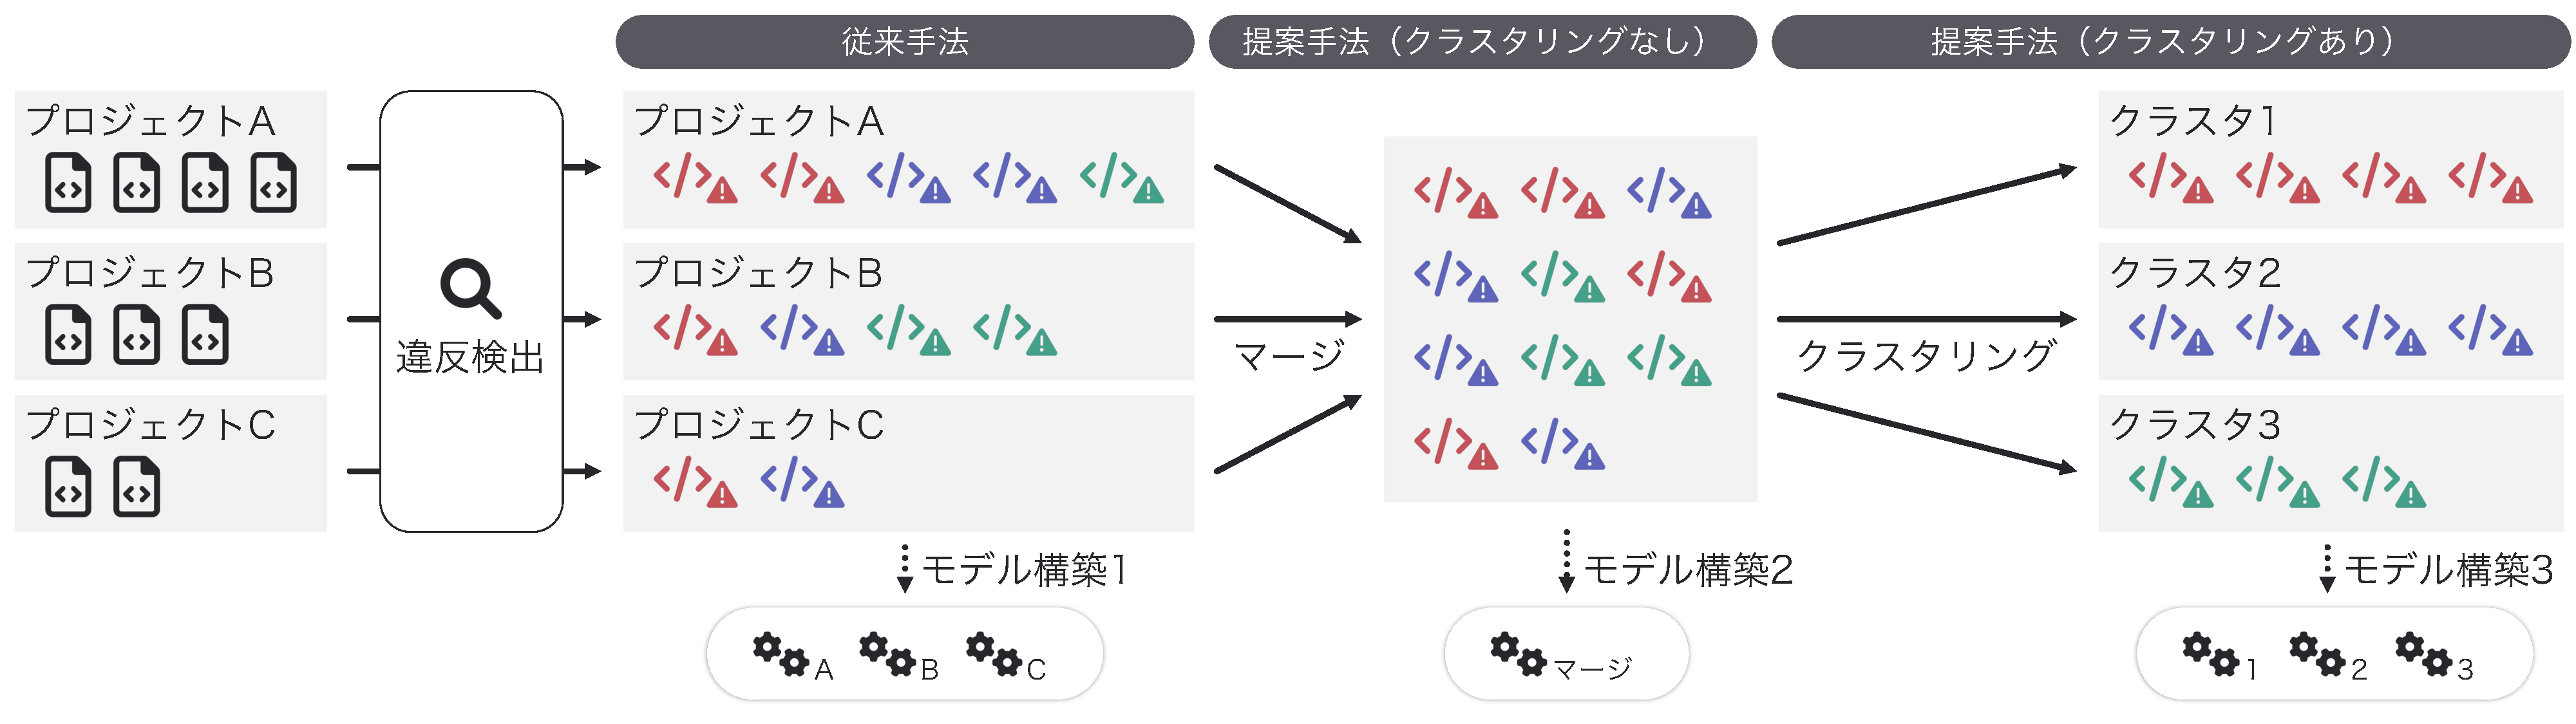
\includegraphics[width=0.8\linewidth]{fig/kameoka_fig1.pdf}
	\caption{本研究の概略図}
	\label{fig:Teiannsyuhou}
\end{figure*}

% \todo{図の更新}図\ref{fig:Teiannsyuhou}は本研究の提案手法を評価するための検証手法を示す.本研究では,静的解析ツールによって検出されたコーディング規約違反を修正すべき違反かそうでない違反かの2値に分類する機械学習モデルを3種類作成する.
\todo{図の更新}図\ref{fig:Teiannsyuhou}に本研究における機械学習モデルの構築と評価の概要を示す.本研究では,静的解析ツールによって検出されたコーディング規約違反を修正が必要な違反かそうでない違反かの2値に分類する機械学習モデルを3種類作成する.

\begin{enumerate}
  \item 単一学習(従来手法):従来研究の手法を採用したモデルであり,予測対象のプロジェクトの過去の規約違反修正履歴のみを学習する予測モデルを構築\cite{JyuraiPre}
  \item 全学習(提案手法):複数プロジェクトの規約違反修正履歴を学習させる手法で,すべてのプロジェクトの学習データを結合し,学習する予測モデルを構築
  \item 選定学習(提案手法):複数プロジェクトの規約違反修正履歴を学習させるが,予測対象プロジェクトと規約違反の修正傾向の似たものだけを学習する予測モデルを構築
\end{enumerate}

モデル(2)では,データセット内のすべてのプロジェクトのデータを学習する.そのため,プロジェクトごとのコーディングスタイルを無視した学習を行う.コーディングスタイルの異なるプロジェクトのデータは学習のノイズとなり,予測精度が低下する恐れがある.しかし,規約違反の修正予測の分野において複数プロジェクトのデータを学習に用いる手法は提案されていないため,モデル(2)の評価が必要である.

モデル(3)の選定学習において,予測対象のプロジェクトと規約違反の修正傾向の類似したプロジェクトのみを学習させる理由は,学習させるデータとして不適切なデータを取り除くためである.モデル(2)で懸念点としてあげたように,単純に全てのプロジェクトの修正履歴のデータを学習させた場合,予測対象のプロジェクトとは異なる修正傾向をしているデータを学習することが考えられる.そのため,予測対象以外の修正履歴を学習データに使用するには,ノイズとなるデータを削減するため修正傾向の似たプロジェクトのデータのみを利用する必要がある.
また,選定学習では,コーディング規約違反の修正傾向の似たプロジェクトのみを収集するために類似度の測定を行っている.類似度の測定時に,欠損値補完を用いる方法と,用いない方法の2種類を検証する.



モデル(1)から(3)を構築,予測結果の評価を行うことで,コーディング規約違反の修正要否予測における,複数プロジェクトを学習に用いることの有効性を明らかにする.



\subsection{説明変数・目的変数の計測方法}


%-------------------------
\begin{figure}[t]
	\centering
	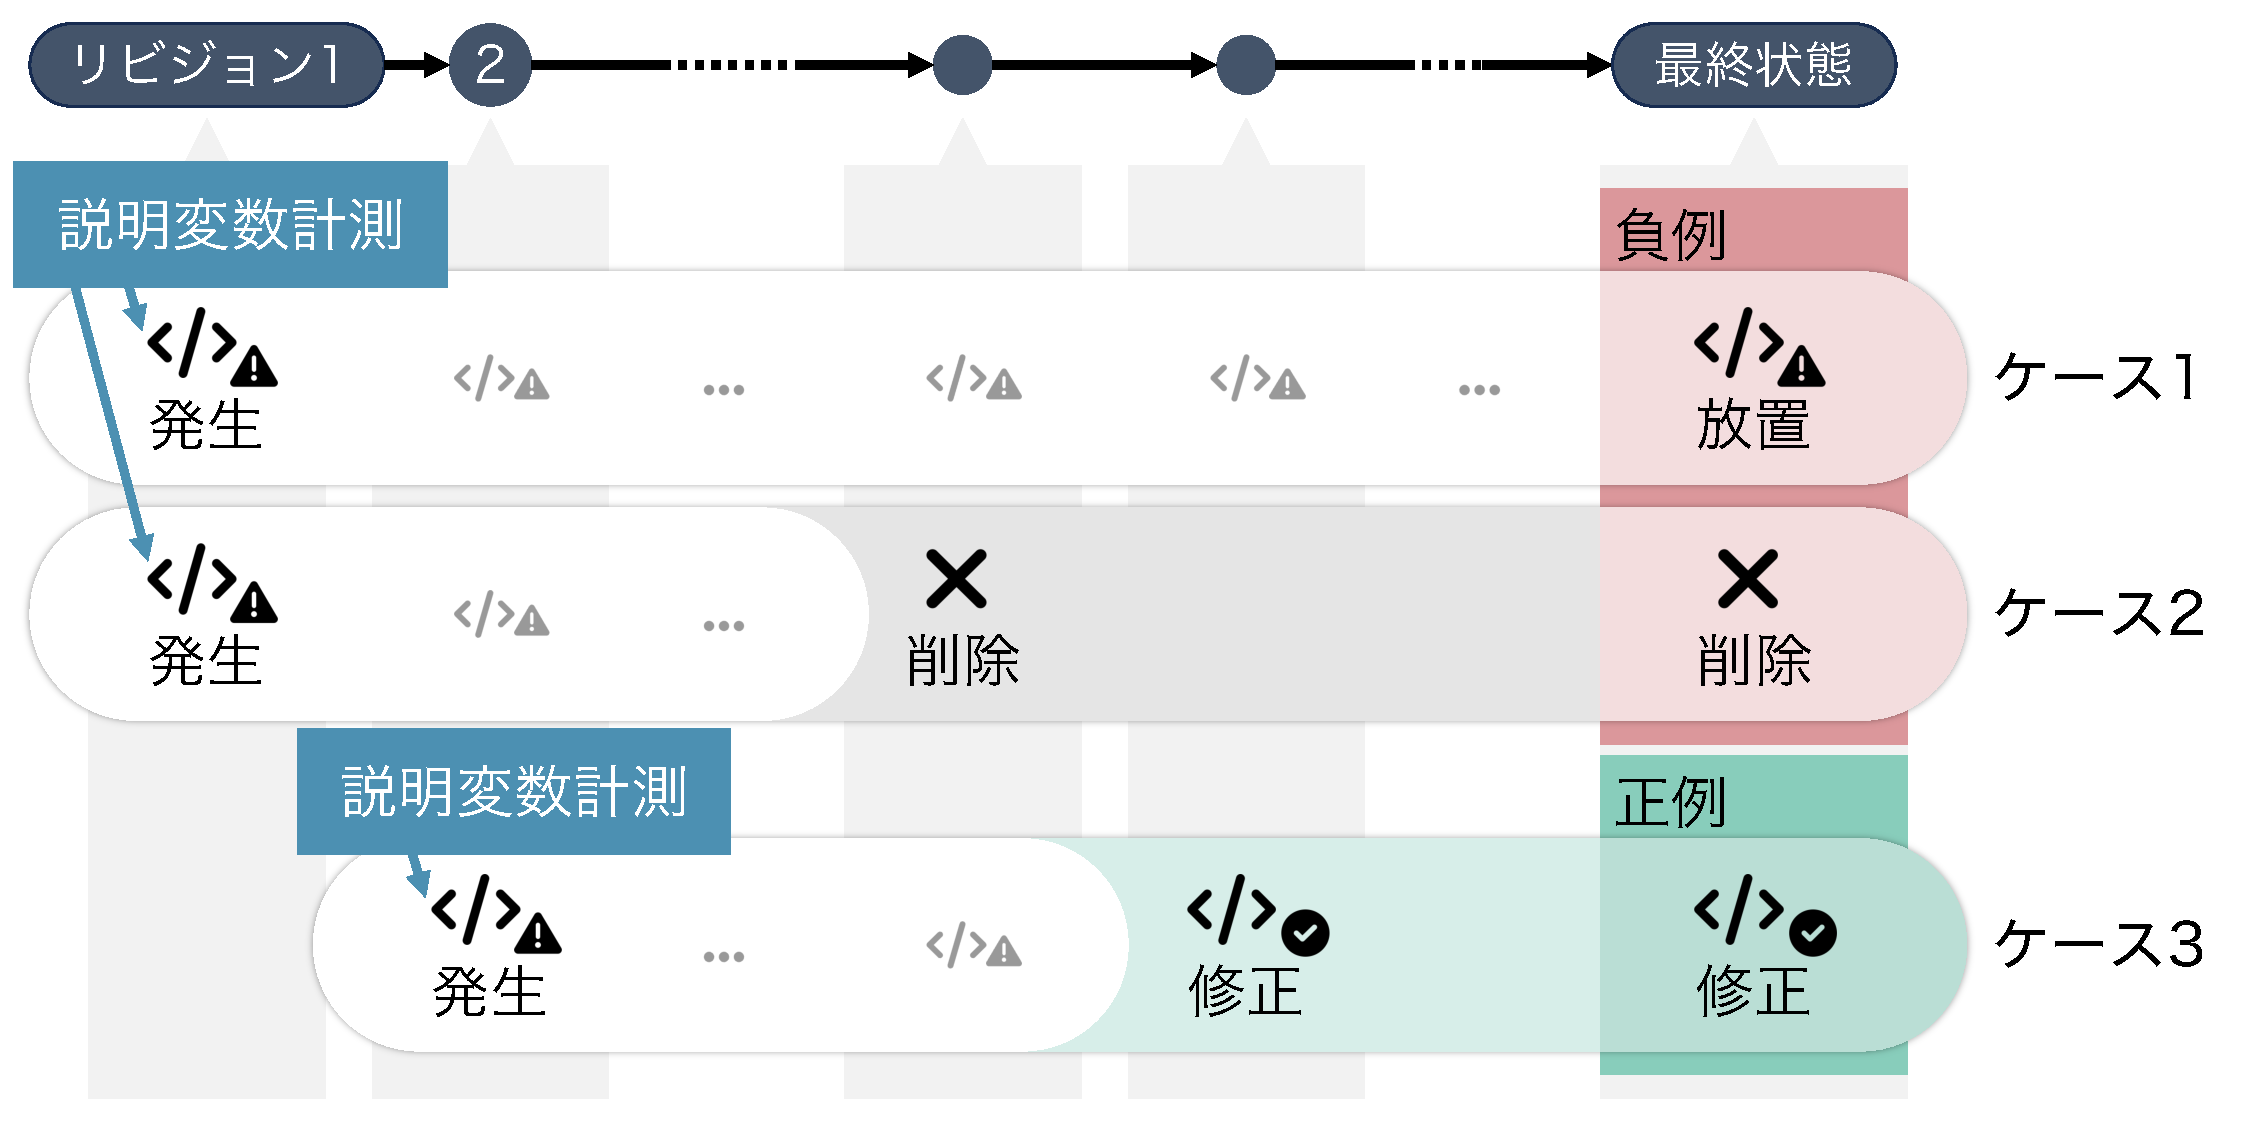
\includegraphics[width=1.0\linewidth]{fig/kameoka_fig2.pdf}
    % \includegraphics[width=0.25\textwidth, bb=0 0 4 3]{fig/fig2.pdf}
	\caption{説明変数と目的変数の計測方法}
	\label{fig:mokutekihensu}
\end{figure}
%-------------------------

図\ref{fig:mokutekihensu}に本研究における説明変数と目的変数の計測位置と,計測方法を示す.本研究では,規約違反の修正履歴から静的解析ツールによって初めて違反が検出された場所を説明変数の計測地点とし,違反コードの最終状態によって,目的変数を計測する.
目的変数の計測についてケースごとにまとめたものが表\ref{tab:pos_neg}である.
図\ref{fig:mokutekihensu}と表\ref{tab:pos_neg}に示すケース1からケース3はそれぞれ対応する同じ事象を示す.
説明変数は,ソースコードの特徴量であるコード行数,コメント行数,循環的複雑度などを含むソースコードに関する特徴量43種類に,コーディング規約違反IDをOne-hotベクトル化したものを加えた合計44種類の特徴量を使用する.ソースコードの特徴量の取得にはテクマトリックス株式会社が開発する静的解析ツールUnderstandを用いて計測する.

%----------------------
\begin{table}[t]
    \centering
    \caption{正例と負例の分類}
    \label{tab:pos_neg}
    \scalebox{0.85}{
    \begin{tabular}{l|l}
         \hline
            分類 & 説明\\ \hline
            負例(ケース1) & コーディング規約の違反が放置されているコード断片\\
            負例(ケース2) & コーディング規約に違反していたコード断片が削除された\\
            正例(ケース3) & コーディング規約に違反していたコード断片が修正された\\
         \hline
    \end{tabular}
    }
\end{table}
%-----------------------

\subsection{機械学習モデルの構築と評価}

本研究で利用する予測アルゴリズムは,離散値を利用する2値分類に協力なRandomForestを用いる.
従来の研究でも明らかにされているように,コーディング規約違反の修正に関するデータは,違反が修正された正例が少なく,修正されない負例が多い不均衡なデータであるため,各予測モデルを構築するためのPythonパッケージに用意されているオプションであるclass\_weightsを用いることによって,2クラスデータに重みづけを行う.
また,学習の反復回数を定めるイテレーション回数を10,000に設定する.

\todo{選定学習の類似度測定方法}

%%%%%%%%%%%%%%%%%%%%%%%%%%%
\section{評価実験}\label{chap:result}
%%%%%%%%%%%%%%%%%%%%%%%%%%%

\subsection{データセット}

% \begin{figure}[t]
% 	\centering
%     % 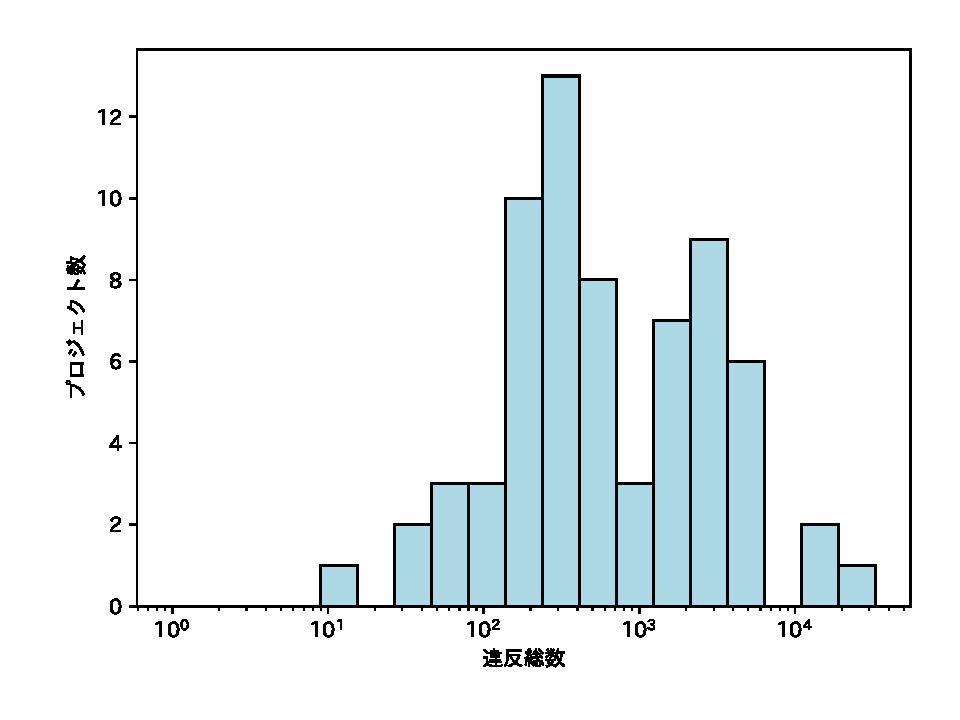
\includegraphics[width=0.25\textwidth, bb=0 0 4 3]{fig/dataset_hist.pdf}
% 	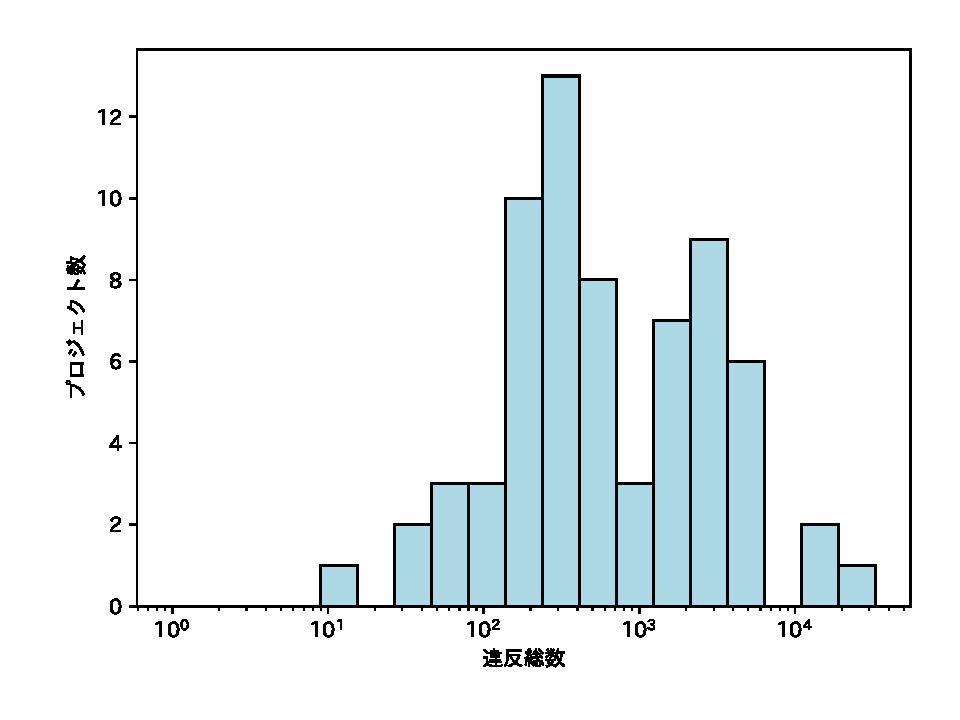
\includegraphics[width=1\linewidth]{fig/dataset_hist.pdf}
% 	\caption{データセットに含まれるプロジェクトごとの違反総数のヒストグラム}
% 	\label{fig:dataset}
% \end{figure}

% \subsubsection{対象プロジェクトの選定方法}
% 本研究ではケーススタディとして,OSSライブラリ検索サービスであるLibraries.io\footnote{Libraries.io: \url{https://libraries.io/}}からPython言語で実装され,静的解析ツールPylintを開発に使用しており,GitHubにソフトウェア,および規約違反修正履歴を公開しているプロジェクトを対象とする.
% 特に,Libraries.ioにおいてOSSの人気度合いや活発度合いを示すSourceRankの上位1,500プロジェクトから静的解析ツールの設定ファイル(pylintrc,または.pylintrc)を保有する81プロジェクトの内,取得した目的変数を学習用データと検証用データに分割した際に,どちらのデータにも正例と負例を含む68プロジェクトを対象とする.

% 本研究では,各分析対象プロジェクトにおいて,2018年12月から1,000日間のコミット履歴を分析対象とする.図\ref{fig:dataset}に,各プロジェクトの総コーディング規約違反数をヒストグラムで示す.図の横軸はプロジェクトごとの総違反数対数軸で示す.違反数が100から1,000のプロジェクトが最も多い.

% \subsubsection{実験結果}

% \begin{table*}[t]
%     \centering
%     \caption{各手法による評価指標で最も高い値で予測したプロジェクト数の一覧}
%     \label{tab:gen}
%     \scalebox{0.9}{
%             \begin{tabular}{l|p{7em}p{7em}p{7em}|p{7em}p{7em}p{7em}}
%             \hline
%             \multirow{2}{*}{手法}&\multicolumn{3}{c|}{{ロジスティック回帰}} & \multicolumn{3}{c}{RandomForest} \\ \cline{2-7}
%              & \multicolumn{1}{r}{{適合率}} & \multicolumn{1}{r}{{再現率}} & \multicolumn{1}{r|}{{F1値}} & \multicolumn{1}{r}{{適合率}} & \multicolumn{1}{r}{{再現率}} & \multicolumn{1}{r}{{F1値}} \\ \hline
%             従来手法 & \multicolumn{1}{r}{{48}} & \multicolumn{1}{r}{{27}} & \multicolumn{1}{r|}{{38}} & \multicolumn{1}{r}{{28}} & \multicolumn{1}{r}{{43}} & \multicolumn{1}{r}{{37}} \\
%             % 提案手法(クラスタリングなし) & 12 & 40 & 18 & 27 & 35 & 23 & 17 & 25 & 18 \\
%             提案手法(クラスタリングなし) & \multicolumn{1}{r}{{12}} & \multicolumn{1}{r}{{40}} & \multicolumn{1}{r|}{{18}} & \multicolumn{1}{r}{{27}} & \multicolumn{1}{r}{{35}} & \multicolumn{1}{r}{{23}} \\
%             % 提案手法(クラスタリングあり) & 20 & 22 & 19  & 28 & 24 & 16 & 24 & 36 & 26 \\ \hline
%             提案手法(クラスタリングあり) & \multicolumn{1}{r}{{20}} & \multicolumn{1}{r}{{22}} & \multicolumn{1}{r|}{{19}}  & \multicolumn{1}{r}{{28}} & \multicolumn{1}{r}{{24}} & \multicolumn{1}{r}{{16}} \\ \hline
%             % 重複数 & 12 & 21 & 7 & 15 & 34 & 8 & 9 & 17 & 4 \\ \hline
%             重複数 & \multicolumn{1}{r}{{12}} & \multicolumn{1}{r}{{21}} & \multicolumn{1}{r|}{{7}} & \multicolumn{1}{r}{{15}} & \multicolumn{1}{r}{{34}} & \multicolumn{1}{r}{{8}} \\ \hline
%         \end{tabular}
%     }
% % \end{table*}
%     \vspace{3mm}
% % \begin{table*}{}
%     \centering
%     \caption{RandomForestモデルでの予測結果(総違反数の上位20件を掲載)}
%     \label{tab:RandomForest}
%     \vspace{1mm}
%     \scalebox{0.9}{
%     \begin{tabular}{l|rrr|rrr|rrr}
%     \hline
%     \multicolumn{1}{c|}{\multirow{2}{*}{プロジェクト名}} & \multicolumn{3}{c|}{従来手法} & \multicolumn{3}{c|}{\begin{tabular}[c]{@{}c@{}}提案手法\\ (クラスタリングなし)\end{tabular}} & \multicolumn{3}{c}{\begin{tabular}[c]{@{}c@{}}提案手法\\ (クラスタリングあり)\end{tabular}} \\ \cline{2-10} 
%     \multicolumn{1}{c|}{} & \multicolumn{1}{c|}{適合率} & \multicolumn{1}{c|}{再現率} & \multicolumn{1}{c|}{F1値} & \multicolumn{1}{c|}{適合率} & \multicolumn{1}{c|}{再現率} & \multicolumn{1}{c|}{F1値} & \multicolumn{1}{c|}{適合率} & \multicolumn{1}{c|}{再現率} & \multicolumn{1}{c}{F1値} \\ \hline
%     sockeye & \multicolumn{1}{r|}{0.75} & \multicolumn{1}{r|}{\textbf{0.83}} & \textbf{0.79} & \multicolumn{1}{r|}{\textbf{0.76}} & \multicolumn{1}{r|}{0.79} & 0.78 & \multicolumn{1}{r|}{\textbf{0.76}} & \multicolumn{1}{r|}{0.80} & 0.78 \\
%     coretools & \multicolumn{1}{r|}{\textbf{0.14}} & \multicolumn{1}{r|}{0.24} & \textbf{0.18} & \multicolumn{1}{r|}{0.04} & \multicolumn{1}{r|}{\textbf{0.41}} & 0.08 & \multicolumn{1}{r|}{0.04} & \multicolumn{1}{r|}{0.37} & 0.07 \\
%     howdoi & \multicolumn{1}{r|}{\textbf{0.78}} & \multicolumn{1}{r|}{\textbf{0.99}} & \textbf{0.87} & \multicolumn{1}{r|}{0.07} & \multicolumn{1}{r|}{\textbf{0.99}} & 0.13 & \multicolumn{1}{r|}{0.07} & \multicolumn{1}{r|}{\textbf{0.99}} & 0.13 \\
%     schema\_salad & \multicolumn{1}{r|}{\textbf{0.66}} & \multicolumn{1}{r|}{\textbf{0.58}} & \textbf{0.62} & \multicolumn{1}{r|}{0.58} & \multicolumn{1}{r|}{0.31} & 0.41 & \multicolumn{1}{r|}{0.46} & \multicolumn{1}{r|}{0.21} & 0.29 \\
%     serverless-application-model & \multicolumn{1}{r|}{\textbf{0.72}} & \multicolumn{1}{r|}{\textbf{0.27}} & \textbf{0.39} & \multicolumn{1}{r|}{0.70} & \multicolumn{1}{r|}{0.23} & 0.34 & \multicolumn{1}{r|}{0.63} & \multicolumn{1}{r|}{0.24} & 0.35 \\
%     SoCo & \multicolumn{1}{r|}{0.67} & \multicolumn{1}{r|}{\textbf{0.64}} & \textbf{0.66} & \multicolumn{1}{r|}{\textbf{0.74}} & \multicolumn{1}{r|}{0.53} & 0.62 & \multicolumn{1}{r|}{0.72} & \multicolumn{1}{r|}{0.47} & 0.57 \\
%     behave & \multicolumn{1}{r|}{\textbf{0.33}} & \multicolumn{1}{r|}{0.37} & \textbf{0.35} & \multicolumn{1}{r|}{0.24} & \multicolumn{1}{r|}{0.36} & 0.29 & \multicolumn{1}{r|}{0.27} & \multicolumn{1}{r|}{\textbf{0.40}} & 0.32 \\
%     OWSLib & \multicolumn{1}{r|}{\textbf{0.61}} & \multicolumn{1}{r|}{\textbf{0.77}} & \textbf{0.68} & \multicolumn{1}{r|}{0.59} & \multicolumn{1}{r|}{0.76} & 0.67 & \multicolumn{1}{r|}{0.58} & \multicolumn{1}{r|}{0.76} & 0.65 \\
%     pynput & \multicolumn{1}{r|}{0.34} & \multicolumn{1}{r|}{\textbf{0.87}} & 0.49 & \multicolumn{1}{r|}{0.55} & \multicolumn{1}{r|}{0.60} & \textbf{0.57} & \multicolumn{1}{r|}{\textbf{0.56}} & \multicolumn{1}{r|}{0.56} & 0.56 \\
%     schematics & \multicolumn{1}{r|}{0.44} & \multicolumn{1}{r|}{0.75} & 0.55 & \multicolumn{1}{r|}{\textbf{0.46}} & \multicolumn{1}{r|}{\textbf{0.79}} & \textbf{0.58} & \multicolumn{1}{r|}{0.43} & \multicolumn{1}{r|}{0.77} & 0.55 \\
%     hickle & \multicolumn{1}{r|}{0.14} & \multicolumn{1}{r|}{0.14} & 0.14 & \multicolumn{1}{r|}{\textbf{0.24}} & \multicolumn{1}{r|}{\textbf{0.49}} & \textbf{0.32} & \multicolumn{1}{r|}{\textbf{0.24}} & \multicolumn{1}{r|}{0.44} & 0.31 \\
%     python-sdk & \multicolumn{1}{r|}{0.43} & \multicolumn{1}{r|}{0.45} & 0.44 & \multicolumn{1}{r|}{0.32} & \multicolumn{1}{r|}{\textbf{0.64}} & 0.43 & \multicolumn{1}{r|}{\textbf{0.45}} & \multicolumn{1}{r|}{0.60} & \textbf{0.52} \\
%     rtv & \multicolumn{1}{r|}{\textbf{0.73}} & \multicolumn{1}{r|}{\textbf{0.51}} & \textbf{0.60} & \multicolumn{1}{r|}{0.72} & \multicolumn{1}{r|}{\textbf{0.51}} & \textbf{0.60} & \multicolumn{1}{r|}{0.65} & \multicolumn{1}{r|}{0.31} & 0.42 \\
%     datadogpy & \multicolumn{1}{r|}{0.02} & \multicolumn{1}{r|}{0.05} & 0.03 & \multicolumn{1}{r|}{0.19} & \multicolumn{1}{r|}{\textbf{0.77}} & 0.31 & \multicolumn{1}{r|}{\textbf{0.24}} & \multicolumn{1}{r|}{0.74} & \textbf{0.36} \\
%     pychromecast & \multicolumn{1}{r|}{\textbf{0.93}} & \multicolumn{1}{r|}{\textbf{0.89}} & \textbf{0.91} & \multicolumn{1}{r|}{0.85} & \multicolumn{1}{r|}{0.76} & 0.80 & \multicolumn{1}{r|}{0.87} & \multicolumn{1}{r|}{0.76} & 0.81 \\
%     pyscard & \multicolumn{1}{r|}{\textbf{0.08}} & \multicolumn{1}{r|}{0.17} & \textbf{0.11} & \multicolumn{1}{r|}{0.06} & \multicolumn{1}{r|}{\textbf{0.50}} & 0.10 & \multicolumn{1}{r|}{0.06} & \multicolumn{1}{r|}{\textbf{0.50}} & \textbf{0.11} \\
%     imgaug & \multicolumn{1}{r|}{0.10} & \multicolumn{1}{r|}{\textbf{0.05}} & \textbf{0.07} & \multicolumn{1}{r|}{\textbf{0.50}} & \multicolumn{1}{r|}{0.02} & 0.03 & \multicolumn{1}{r|}{\textbf{0.50}} & \multicolumn{1}{r|}{0.02} & 0.03 \\
%     GPflow & \multicolumn{1}{r|}{0.64} & \multicolumn{1}{r|}{\textbf{0.89}} & \textbf{0.74} & \multicolumn{1}{r|}{0.55} & \multicolumn{1}{r|}{0.20} & 0.29 & \multicolumn{1}{r|}{\textbf{0.66}} & \multicolumn{1}{r|}{0.22} & 0.33 \\
%     transitions & \multicolumn{1}{r|}{\textbf{0.83}} & \multicolumn{1}{r|}{0.96} & \textbf{0.89} & \multicolumn{1}{r|}{0.81} & \multicolumn{1}{r|}{\textbf{0.98}} & \textbf{0.89} & \multicolumn{1}{r|}{0.82} & \multicolumn{1}{r|}{\textbf{0.98}} & \textbf{0.89} \\
%     pyphi & \multicolumn{1}{r|}{0.67} & \multicolumn{1}{r|}{0.78} & 0.72 & \multicolumn{1}{r|}{\textbf{0.69}} & \multicolumn{1}{r|}{\textbf{0.92}} & \textbf{0.79} & \multicolumn{1}{r|}{\textbf{0.69}} & \multicolumn{1}{r|}{\textbf{0.92}} & \textbf{0.79} \\ \hline
%     \end{tabular}
%     }
%     \vspace{3mm}
% \end{table*}

%%%%%%%%%%%%%%%%%%%%%%%%%%%
\section{考察}\label{chap:consideration}
%%%%%%%%%%%%%%%%%%%%%%%%%%%


%%%%%%%%%%%%%%%%%%%%%%%%%%%
\section{妥当性への脅威}\label{chap:heuristic}
%%%%%%%%%%%%%%%%%%%%%%%%%%%
\subsection{内的妥当性}


% 目的変数の計測において,規約違反しているコードが修正された場合のみ正例として扱い,削除された場合は,修正されたわけではないため本研究では負例として扱っている.しかし,コーディング規約違反の中には該当部分を削除することによっても解消するものがあるため,本来正例として扱うべきケースを負例として計測してしまっていることがある.
% コードの移動に関してもGitHubの仕様上,削除と追加という扱いになるため,コードの移動によってコーディング規約に違反しているコードが削除され不例として計測している可能性がある.
% また,コーディング規約に違反しているコードが,可読性とは関係のない実行速度などの観点からコードが修正された場合でも,違反していたコードが削除された場合は不例として計測してしまっている.


% 本研究で用いた2種類の機械学習アルゴリズム以外にも,より正確な予測を可能にするアルゴリズムが存在する可能性がある.
% それぞれのパラメータの更新回数である,イテレーション回数を10,000に設定したが,データサイズが大きいプロジェクトではモデルが収束しないことが確認された.モデルが収束しない場面も確認されたが,本研究で主に用いた実験環境とは別の環境で,複数回実行した場合でも予測結果に変化はなかったので,モデルが収束しない問題に関しては,本研究の結果に対して大きな影響を与える可能性は低い.


\subsection{外的妥当性}

本研究ではケーススタディとしてPython言語を主な開発言語としたプロジェクト68件の規約違反修正履歴を収集して検証を行った.
また,プロジェクト数をさらに拡張した場合や,対象とするプロジェクトや期間を変更した場合に予測精度が変化することが示唆される.
対象言語をPython以外の言語とした場合予測結果が変化することが示唆される.
しかし,本研究で使用したデータセットは68プロジェクトでプロジェクトごとのデータ数が中央値で500.5件のデータ数を含んでいるので,更なるデータサイズの拡張による予測精度への影響は低いと考えられる.



%%%%%%%%%%%%%%%%%%%%%%%%%%%
\section{おわりに}\label{chap:end}
%%%%%%%%%%%%%%%%%%%%%%%%%%%

% 本研究では,静的解析ツールによってソースコード中に含まれるコーディング規約違反を検出した結果から,修正すべき違反か否かに分類するタスクにおいて予測対象プロジェクト以外の開発データも予測モデルの学習に用いた場合の予測結果への影響を調査した.結果として,ロジスティック回帰モデル,RandomForestモデルの2種類のモデル構築手法において,従来手法である予測対象プロジェクトの過去の規約違反修正履歴のみを学習した場合が,提案手法より多いプロジェクトで高いF1値で修正予測が可能であった.しかし,予測対象プロジェクト以外の開発データも学習する提案手法(クラスタリングなし),提案手法(クラスタリングあり)によって検証に使用した68プロジェクトの1/4程度ずつのプロジェクトでF1値の向上を確認した.
% F1値が向上した理由として,データセットを拡張したことによる,モデルの最適化によって予測精度が向上したことが示唆される.しかし,違反しているコーディング規約の種類が他プロジェクトに比べて特徴的な場合,不必要なデータを学習してしまい,予測精度が低下することも確認した.

% 本研究において複数プロジェクトを学習に用いる提案手法によって予測精度が向上するプロジェクトを確認することができたので,各プロジェクトごとに違反しているコーディング規約の特徴ごとにグループ化し,各グループごとに学習することによって,コーディング規約違反の修正予測精度の向上を見込むことができる.

% \ack %% 謝辞

%\bibliographystyle{sieicej}
%\bibliography{myrefs}
\bibliographystyle{sieicej}
\bibliography{Kameoka}
% \begin{thebibliography}{99}% 文献数が10未満の時 {9}
% \bibitem{}
% \end{thebibliography}

\appendix
\section{}

%% 著者紹介・顔写真の掲載はC分冊の場合は任意です.
\begin{biography}
\profile{n}{亀岡 令}{サンプル}
%\profile{会員種別}{名前}{紹介文}% 顔写真あり
%\profile*{会員種別}{名前}{紹介文}% 顔写真なし
\end{biography}

\end{document}
